\graphicspath{{images/methodology/}}
\section{Reinforcement learning method}
The reinforcement learning method trains an agent to take the optimal sequence of decisions \cite{sutton2018reinforcement}. The learning process uses positive and negative reinforcement to increase or decrease the probability of choosing an specific action. In this sense, the agent learns, through an iterative process, to make the sequence of decisions that maximizes the amount of reward that he will receive \cite{sutton2018reinforcement}.

The framework of reinforcement learning is formed by four elements: (i) agent, (ii) actions, (iii) environment, and (iv) states and rewards \cite{sutton2018reinforcement}. Figure \ref{fig:RL_framework} describes the reinforcement learning framework for the application that a mobile robot must reach the desired position. First, an agent is the entity who takes decisions based on the reward and punishment that he will receive. Second, action space are all the available actions that the agent could use to interact with the environment. Third, the environment is the space where the agent lives and interact. Fourth,  the new agent's state after applying an action in the environment and the reward associated with that specific action. This process will be repeated several times until the agent learns a successful strategy to interact with the environment and maximize the reward.

In reinforcement learning, the agent's strategies are called policies and indicate which actions the agent should chooses in each state \cite{sutton2018reinforcement}. Policies are usually stochastic to consider the uncertainties and probabilities of real world \cite{tedrake2004stochastic}.  In this way, policies assign a probability to each action and the agent chooses the action with the highest probability. Hence, the objective of reinforcement learning algorithms is find the optimal policy that maximize the amount of reward. 

A standard

\begin{figure}[t!]
	\centering
	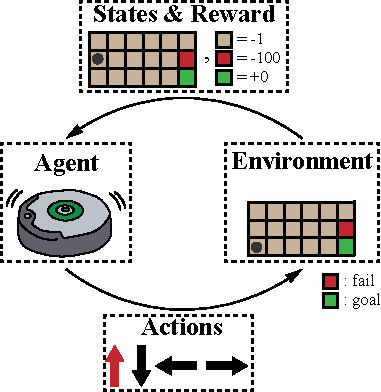
\includegraphics{reinforcement_learning_diagram.pdf}
	\caption{Reinforced learning framework for the application that a mobile robot must reach the desired position. In this example, the agent's actions are up, down, right and left; likewise, the agent's objective is reach the green cell and the agent fails when reach the red cell.}
	\label{fig:RL_framework}
\end{figure}

\section{Deep reinforcement learning}

%the development of a bipedal robot controller, made in the simulator for multi-body dynamics MuJoCo, with the use of the deep reinforcement learning algorithms class Proximal Policy Optimization (PPO). In addition, an analysis will be carried out on the joints of the robots to understand the degree of importance of each one of them in the gait learning process.


%based on reward or punish an specific behavior \cite{sutton2018reinforcement}. In this way, the model take decisions/actions and learn through trial and error. The framework is formed by four parts: (i) agent, (ii) action, (iii) environment and (iv) reward. This learning method maintains growing interest in development due to its simplicity and powerful problem-solving capabilities.

